\chapter{Konfigurationsraum} \label{ch:config-space}
Bei einer Roboterlänge und -breite größer als eins können gewisse Punkte im Occupancy Grid nicht erreicht werden, ohne Hindernisse oder Grenzen zu überdecken. 
Deshalb wird die Roboterbewegung im \textit{Konfigurationsraum} in eine Punktbewegung (\texttt{robot\_width = robot\_length = 1}) transformiert.
Dazu wird jedes Hindernis im Occupancy Grid um die Roboterdimensionen erweitert. \cite{roberts.1999}

Je nach Rotation ändern sich die überdeckten Koordinaten im Occupancy Grid.
Um den Verbrauch freier Koordinaten um das Hindernis zu minimieren, unterteilen Yunfeng und Chirikjian die Rotation in diskrete Zustände \cite{wang.2000}. Die Variable \texttt{rotation\_step} gibt als Teiler von $360$° an, um wie viel Grad sich der Roboter pro Bewegungsschritt drehen kann, wodurch sich \texttt{rotations=360/\texttt{rotation\_step}} unterschiedliche Rotationszustände ergeben.
\begin{figure}[H]
	\centering
	\footnotesize
	\centerline{\resizebox{0.6\linewidth}{!}{\input{bilder/rotation-steps_latex.pdf_tex}}}
	\caption{Für \texttt{rotation\_step=45} ergeben sich $(360 \text{\textdegree} \div 45 \text{\textdegree}) = 8$ Rotationszustände.}
\end{figure}

\vspace*{-0.2cm}
Für jeden Rotationszustand wird ein \textit{erweitertes Occupancy Grid} generiert. Dazu wird eine Maske des Robotermodells erstellt, rotiert und punktgespiegelt. Pro Rotatioszustand wird in einer Kopie des ursprünglichen Occupancy Grids jedes Hindernis sowie jede Grenzkoordinate um diese Maske erweitert.
%\vspace*{0.02cm}
\begin{figure}[H]
	\centering
	\footnotesize
	\centerline{\resizebox{0.97\linewidth}{!}{\input{bilder/robot-mask_latex.pdf_tex}}}
	\caption{Erzeugung eines erweiterten Occupancy Grid für eine Rotation um $45$°}
\end{figure}

Der Konfigurationsraum \texttt{configuration-space[rotation][y][x]} mit den Dimensionen fasst die erweiterten Occupancy Grids in der Dimension \texttt{[rotation]} zusammen:
\begin{itemize}
\item \texttt{(rotation + 1) \% rotations} $\widehat{=}$ Rotation um \texttt{rotation\_step} gegen den Uhrzeigersinn
\item \texttt{(rotation - 1) \% rotations} $\widehat{=}$ Rotation um \texttt{rotation\_step} im Uhrzeigersinn
\end{itemize}
\vspace*{0.4cm}
\begin{figure}[H]
	\centering
	\footnotesize
	\centerline{\resizebox{1\linewidth}{!}{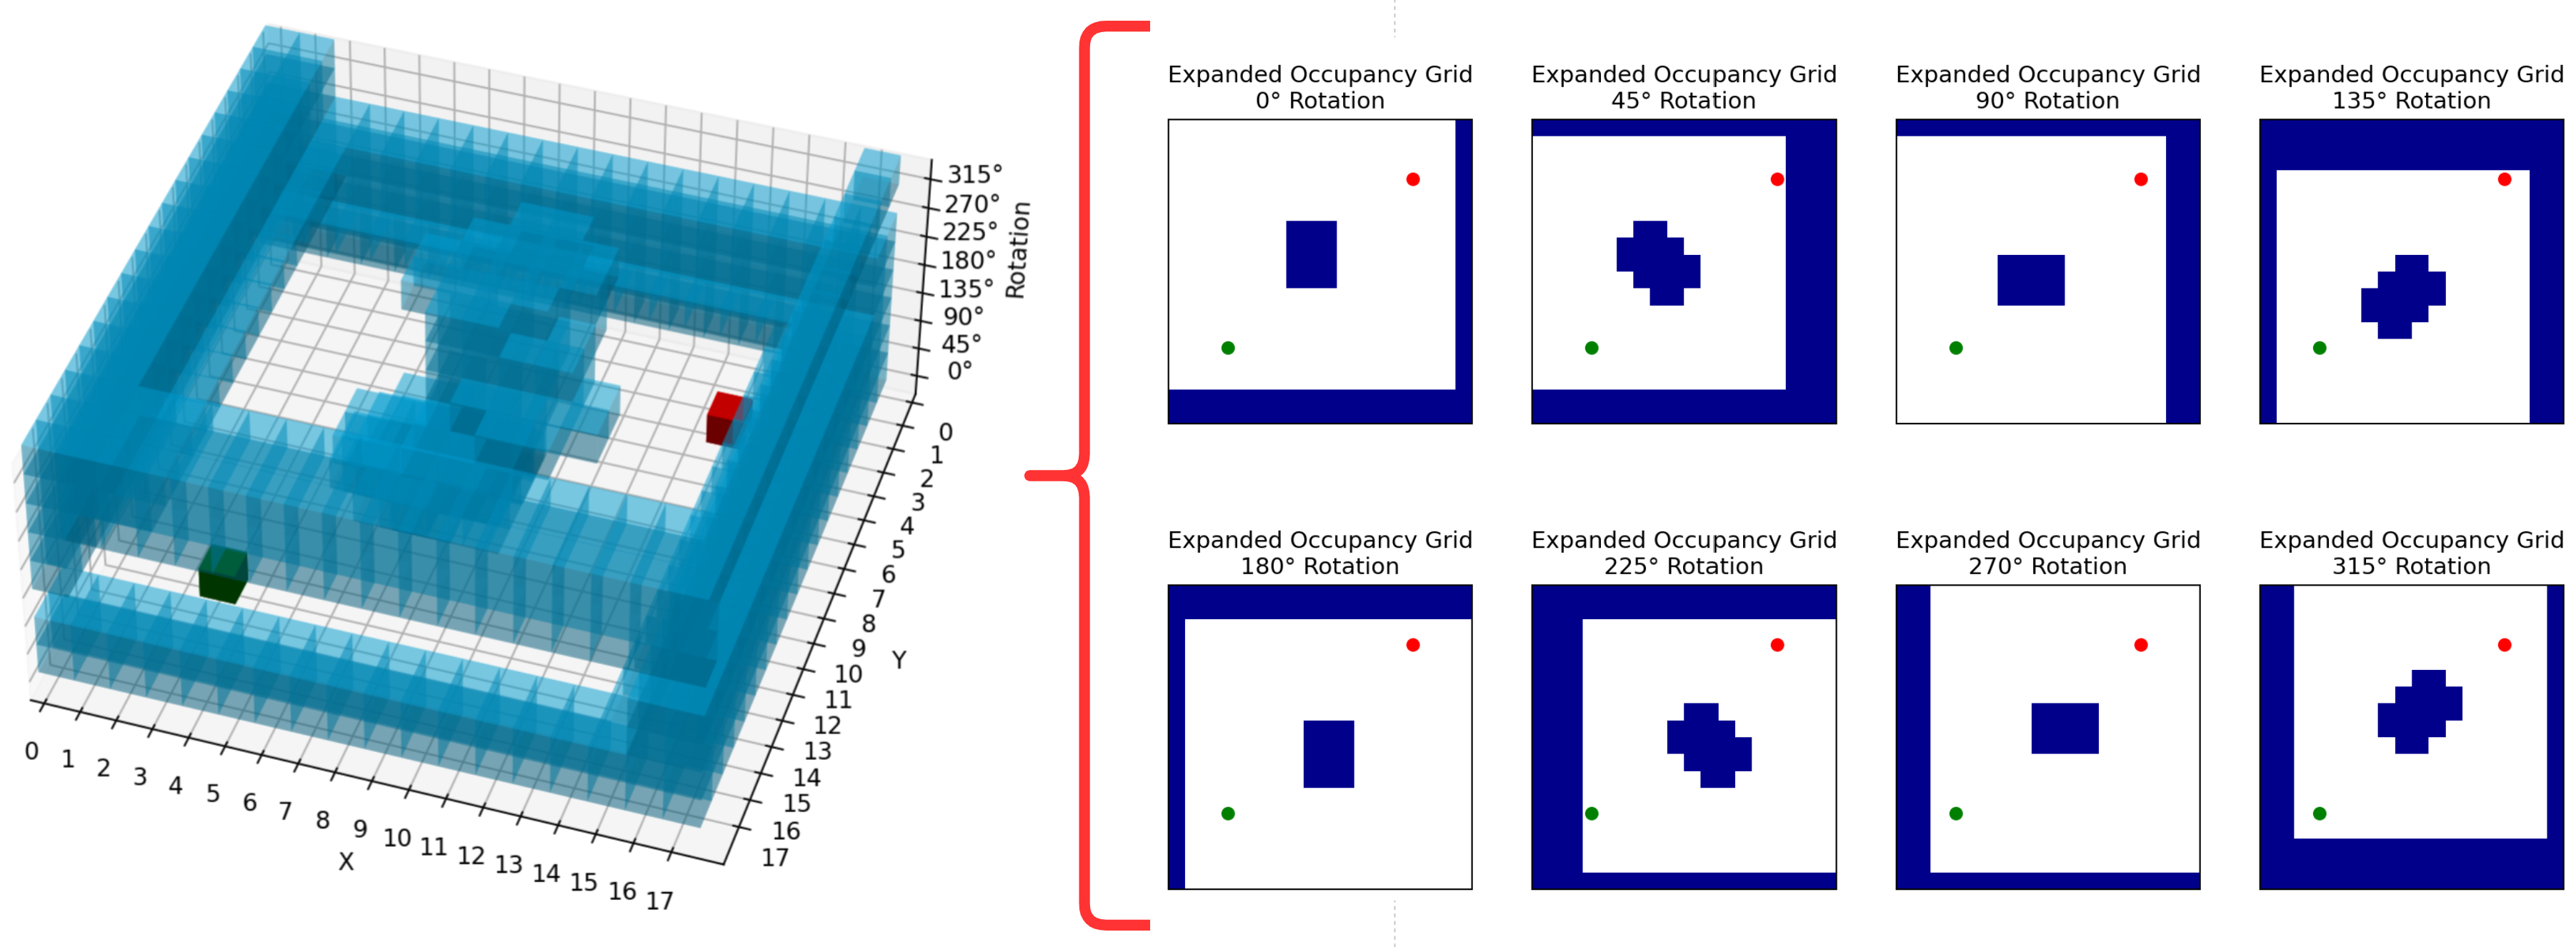
\includegraphics{bilder/configuration-space.png}}}
	\caption{Die erweiterten Occupancy Grids bilden den Konfigurationsraum}
\end{figure}

Der berechnete Konfigurationsraum $\texttt{rotations*occupancy\_grid\_length*occupancy\_grid\_width}$ nach Yunfeng und Chirikjian ermöglicht über die Punktbewegung im dreidimensionalen Raum eine kollisionsfreie Translation und Rotation im Occupancy Grid bei minimalem Verbrauch freier Koordinaten \cite{wang.2000}. 
Die Position des Roboters sowie dessen Rotationszustand im Occupancy Grid wird dabei im Konfigurationsraum über die Dimensionen \texttt{rotation, y, x} referenziert.


